\subsection{Da função de seis zeros às sete portas}
\label{sec:gbp-sete-portas}
\index{circuito aritmetico@circuito aritmético!certificado de divisor@certificado de divisor}

Voltemos à função que construímos com um zero triplo e três zeros
simples, na secção~\ref{sec:divisors-seis-zeros}. Os coeficientes,
as coordenadas e as multiplicidades estão todos à vista do leitor.
Podemos, por isso, acompanhar uma testemunha completa e ao mesmo
tempo descobrir que parte dela precisa de estar à vista de Bob.
Escrevamos a função, com o coeficiente de \(x\) fixo, na forma
\[
       f=a+x+bx^2+cx^3+(d+ex)y .
\]
Alice tem duas listas. A primeira reúne os coeficientes livres
\(\boldsymbol c_f=(a,b,c,d,e)=(10,9,10,9,6)\). A segunda
guarda as cinco multiplicidades e as coordenadas de \(W\), pela ordem
\[
 \boldsymbol c_m=(u_0,u_1,u_2,u_3,u_4,X,Y)
                   =(0,1,3,1,0,10,6).
\]
Cada lista entra num compromisso vectorial, \(K_f\) ou \(K_m\).
Tomemos oito posições em cada um e, para a abertura honesta,
completemos as listas com zeros. A declaração de conhecimento
refere as coordenadas que entram nas suas equações. Escolher este
arranjo permite distinguir as duas listas ao escrever as matrizes.
A prova admite também repartições diferentes. As igualdades
geométricas que se seguem pertencem todas a \(\mathbb F_{17}\), e
a ordem dezanove só regressará quando falarmos do escalar de \(P\).

Suponhamos que a secante pública é \(y=6\). Os seus três encontros
são \(B_0=(0,6)\), \(B_1=(7,6)\) e \(B_2=(10,6)\).
Podemos verificá-los num só cálculo, substituindo a ordenada na
equação da curva. O polinómio obtido é \(x^3+2x+2-36=x^3+2x\)
no corpo. As três raízes são \(0,7,10\), pois
\(7^2=10^2=15=-2\). São distintas. No ponto \(B_2\), que por
acaso coincide com \(W\), \(f(B_2)\) é não nulo. O zero
prescrito no divisor corresponde a \(-W\), na outra ordenada da
mesma fibra. A distinção dos sinais feita na construção da função
tem agora uma consequência visível no denominador.

Com declive zero, \(s=3x^2+2\) é o factor público que entra
no denominador em cada encontro. Aqui, e apenas nas contas
da secante, a letra \(s\) abrevia esse factor. As derivadas
parciais da função são
\[
 f_x=1+2bx+3cx^2+ey,\qquad f_y=d+ex .
\]
Em \((x,6)\), a parcela secreta da prova tem a forma
\[
          o=\frac{N}{D},\qquad N=12 f_x+s f_y,\qquad D=s f .
\]
Tudo o que multiplica um dos cinco coeficientes secretos é conhecido
quando se conhece a secante. Por exemplo, o coeficiente de \(e\)
em \(N\) é \(12\cdot6+sx\), e em \(D\) é \(6sx\).
Bob pode, portanto, escrever uma linha pública para \(N\) e outra
para \(D\) em cada encontro. À esquerda do quadro indicamos o
termo constante e à direita os cinco multiplicadores na ordem
\((a,b,c,d,e)\). A notação \([k\mid\boldsymbol v]\) significa
\(k+\langle\boldsymbol v,\boldsymbol c_f\rangle\).
\[
\begin{array}{c|c|r|rrrrr}
 x& &k&a&b&c&d&e\\ \hline
 0&D&0 &2&0&0&12&0\\
 0&N&12&0&0&0& 2&4\\
 7&D&6 &13&8&5&10&2\\
 7&N&12&0&15&13&13&10\\
10&D&11&13&8&12&10&15\\
10&N&12&0&2&13&13&15
\end{array}
\]
Assim, em \(x=7\), o coeficiente de \(c\) no denominador é
\(s\cdot 7^3=13\cdot3=5\). O coeficiente do mesmo \(c\)
no numerador vale \(12\cdot3\cdot7^2=36\cdot15=13\).
São os números que qualquer verificador obterá com a curva e a
secante deste exemplo. Para calcular o valor de uma das formas
lineares é que entram os números escondidos em \(K_f\).

Alice aplica o quadro à sua primeira lista. No primeiro encontro
encontra \(D_0=2\cdot10+12\cdot9=9\) e
\(N_0=12+2\cdot9+4\cdot6=3\). A inversa de nove vale dois,
pelo que \(o_0=6\). Para os outros encontros, as contas dão
\[
\begin{array}{c|rrr|l}
       &D_r&N_r&o_r&D_ro_r=N_r\pmod{17}\\ \hline
 B_0&9&3 &6&9\cdot6=54=3\\
 B_1&3&12&4&3\cdot4=12\\
 B_2&3&10&9&3\cdot9=27=10
\end{array}
\]
A primeira soma que há-de figurar na prova é, pois,
\(o_0+o_1+o_2=6+4+9=2\). Esta conta partiu dos coeficientes da
função e das três avaliações. A segunda parte do circuito parte
da outra lista e percorre os pontos da tabela.

As ordenadas de \(P,2P,4P,8P,16P\) são \(1,3,1,7,11\).
Os pesos associados à secante horizontal são, pela mesma ordem,
as inversas de \(5,3,5,-1,-5\), isto é,
\[
                         (7,6,7,16,10).
\]
O coeficiente de \(4P\) conta três vezes. O coeficiente de
\(16P\) é zero, mas o ponto \(-W\) tem a mesma ordenada que
\(16P\). A sua contribuição para o lado direito entra pela inversa
\(v_W=(6+Y)^{-1}=12^{-1}=10\). Resulta
\[
       7\cdot0+6\cdot1+7\cdot3+16\cdot1+10\cdot0+10
                       =53=2\pmod{17}.
\]
Temos assim os dois números a comparar. A lista dos zeros conduziu
ao mesmo dois que os coeficientes da função. Ao verificar esta
condição numa prova, Bob conhece os cinco pesos, escolhe a posição
de cada variável e escreve a igualdade que as liga. O número dois
é uma conta que pudemos fazer porque conhecíamos as duas aberturas.

Para escrever estas condições como produtos, chamemos \(L_i\),
\(R_i\) e \(O_i\) às entradas e à saída da porta \(i\), com
\(L_iR_i=O_i\). As duas primeiras colunas de números dão os operandos
e a terceira dá o resultado. A última coluna dá
o significado do produto no circuito.
\begin{center}
\begin{tabular}{c|rrr|l}
 \(i\)&\(L_i\)&\(R_i\)&\(O_i\)&Relação\\ \hline
 1&10&10&15&\(X\cdot X=X^2\)\\
 2&15&10&14&\(X^2\cdot X=X^3\)\\
 3& 6& 6& 2&\(Y\cdot Y=Y^2\)\\
 4& 9& 6& 3&\(D_0 o_0=N_0\)\\
 5& 3& 4&12&\(D_1 o_1=N_1\)\\
 6& 3& 9&10&\(D_2 o_2=N_2\)\\
 7&12&10& 1&\((6+Y)v_W=1\)
\end{tabular}
\end{center}
Bob deve ainda ligar essas portas. A relação \(O_1=L_2\) conduz
o quadrado de \(X\) à segunda multiplicação. As três ocorrências
de \(X\) em \(L_1,R_1,R_2\) apontam para a sexta posição de
\(K_m\), e \(L_3,R_3\) para a sétima. A linha
\(O_3-O_2-2X=2\) conclui a equação da curva. Os valores do
quadro dão \(2-14-20=-32=2\). Antes desta ligação, três produtos
apenas tinham calculado dois quadrados e um cubo. A ligação diz
que o par das coordenadas pertence à curva exigida.

Nas portas quatro a seis, as entradas esquerdas devem ser os
\(D_r\) e as saídas devem ser os \(N_r\). É aqui que as seis
linhas do quadro dos coeficientes entram nas matrizes públicas.
Por exemplo, a entrada esquerda da quinta porta obedece a
\[
      L_5-13a-8b-5c-10d-2e=6.
\]
Qualquer linha como esta custa uma ligação linear, pois cada parcela
usa um coeficiente público. O produto de \(D_1\) com a razão
secreta exige a quinta porta. Na sétima escrevemos
\(L_7-Y=6\) e \(O_7=1\). O seu operando direito passa, assim,
a ser a inversa que a lista de zeros requer. A última ligação toma
a seguinte forma
\[
  R_4+R_5+R_6-R_7-7u_0-6u_1-7u_2-16u_3-10u_4=0 .
\]
Substituindo os valores da tabela recuperamos \(19-10-43=-34=0\).
Estes totais inteiros diferem porque os valores pertencem ao corpo.
A igualdade que a linha exige é a dos seus resíduos.

Dá para ler deste esquema o tamanho do circuito inteiro. Há sete
ligações para as três primeiras portas, contando as duas entradas
de cada uma e a equação da curva. Para as três razões há seis
ligações, para a inversa duas, para a comparação final uma.
São dezasseis linhas lineares e sete multiplicações. Em vectores
de comprimento oito cabe ainda uma porta de preenchimento, para a
qual a testemunha honesta escolhe \(0\cdot0=0\). As restrições que
acabámos de escrever utilizam somente as sete portas assinaladas.
O total de dezasseis pertence a esta maneira de nomear e ligar
os fios. Separar uma soma linear em duas linhas com uma variável
auxiliar daria outra contagem e continuaria a representar a
mesma conta geométrica.

A figura indica a ordem em que Alice pode obter as duas listas de
dados. Nas setas que descem para as portas, a secante já foi
determinada. As incógnitas que representam as razões podem,
portanto, depender dela.
\begin{center}
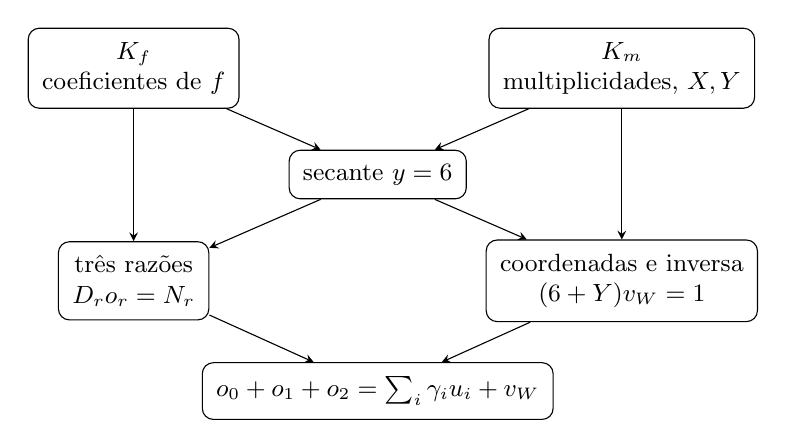
\begin{tikzpicture}[>=stealth,font=\small,
 box/.style={draw,rounded corners,align=center,inner sep=5pt}]
 \node[box] (kf) at (-3.1,0) {\(K_f\)\\coeficientes de \(f\)};
 \node[box] (km) at (3.1,0) {\(K_m\)\\multiplicidades, \(X,Y\)};
 \node[box] (line) at (0,-1.35) {secante \(y=6\)};
 \node[box] (fun) at (-3.1,-2.7) {três razões\\\(D_r o_r=N_r\)};
 \node[box] (point) at (3.1,-2.7) {coordenadas e inversa\\\((6+Y)v_W=1\)};
 \node[box] (sum) at (0,-4.1) {\(o_0+o_1+o_2=\sum_i\gamma_i u_i+v_W\)};
 \draw[->] (kf)--(line); \draw[->] (km)--(line);
 \draw[->] (kf)--(fun); \draw[->] (km)--(point);
 \draw[->] (line)--(fun); \draw[->] (line)--(point);
 \draw[->] (fun)--(sum); \draw[->] (point)--(sum);
\end{tikzpicture}
\end{center}

Temos agora os mesmos ingredientes da prova dos dois quadrados.
Naquela, duas portas e cinco linhas ligavam \(K,V\) ao resultado.
Nesta, as dezasseis linhas referem os dois compromissos vectoriais,
e o lado direito contém apenas constantes públicas. Assim, ao
formar o coeficiente reservado, Bob pode calcular todo o escalar
\(\delta+\langle\boldsymbol z,\boldsymbol b\rangle\) a partir
do circuito e dos desafios. Antes bastava-lhe um compromisso nesse
valor, porque a soma dos quadrados estava guardada em \(V\).
Agora a privacidade reside inteiramente nas duas listas e na
atribuição das portas. Os compromissos e as correcções da segunda
igualdade continuam indispensáveis para ligar o produto interno a
essas mesmas listas.

O exemplo pequeno tem uma vantagem precisa. Podemos acompanhar
cada linha da declaração e calcular os dois membros da igualdade final com os
mesmos dados que a demonstração manteve ocultos. Tem, também, a limitação natural do corpo
que escolhemos para ver os números. No limite probabilístico de
\eqref{eq:gbp-residuos}, dezasseis linhas e apenas dezasseis
desafios não nulos já dão a cota um. As igualdades acima estabelecem
a correcção dos cálculos da testemunha exibida. Para a solidez da
prova usam-se os parâmetros grandes, a vinculação a uma abertura e
as hipóteses de conhecimento estudadas com o protocolo
\cite{eagen-divisors,generalized-bulletproofs-fixed,monero-oxide-fcmp-source}.
